\chapter{Le Stage}
\section{Sujet}

Le sujet de stage est la participation au développement d'une évolution sur l'application Geofibre.
Le client souhaiterais en effet intégrer de nouvelles fonctionnalités, notamment l'intégration des cartes des départements d'Outre-Mer au sein de l'application.
\\Cette version s'annoncant conséquente, l'équipe dirigante a décidé de renforcer le groupe.

\section{Objectif}


L'objectif du stage est, dans un premier temps, de participer aux phases de développement jusqu'à la livraison pour l'évolution prévue sur l'application et dans un second temps de participer à la maintenance de l'application.

\chapter{Organisation de l'équipe}

L'équipe de travail est organisée de la façon suivante :\\

\begin{itemize}
  \item Le chef de groupe
  \item Le chef de projet
  \item L'équipe de développement
  \item Le responsable de test, c'est aussi le chef de projet.
  \item Le responsable du groupe, c'est un membre de l'équipe de développement.
  \item Le responsable du groupe 2, c'est un membre de l'équipe de développement.\\
\end{itemize}
Je suis intégré au sein de l'équipe de développement composée de 10 personnes (1 externe et 9 salariés).
\\Nous fonctionnons suivant la méthode \textit{LEAN}.

 \begin{colbox}{{HTML}{A3E8FF}}{La méthode LEAN\\ }
   \textbf{Objectif} : Améliorer de façon continue la performance en termes de qualité, coûts et délais de livraison.
   \\\textbf{Origine} : Apparue dans le seconde moitié du XXème siècle avec l'entreprise \textit{Toyota}. La production de voiture répond à une demande, ainsi les stocks sont quasi inexistants.
   \\\textbf{Principe} : Créer de la valeur ajoutée pour le client avec un minimum de gaspillage et en livrant un maximum de qualité.
   \\\textbf{En tant que développeur} : Des indicateurs de qualité de code à améliorer au fil des versions, des délais de livraison du service fini à respecter.
 \end{colbox}

 Chaque jour à 9h30 nous avons une réunion (\textit{Daily Meeting}) où chaque membres de l'équipe, tour par tour, décrit son humeur de la veille, les tâches qu'il a réalisé, les problèmes éventuels à signaler et ce qu'il prévoit de faire au fil de la journée.
 \\ C'est une méthode qui permet de savoir où en est le projet, et plus particuliéremment chaque membres de l'équipe. \\Cette méthode permet aussi de chercher les solutions ensemble aux problèmes et affecter plus de personnes sur une tâche bloquante dans la limite du possible.
\\La communication et la transparence sur le travail réalisé font que les problèmes ne restent pas longtemps sans solutions.
\\De plus, l'aménagement de l'\textit{Open-Space} permet de demander de l'aide rapidement aux collègues de travail. Ca permet de ne pas rester bloquer sur une tâche ou se désorienter.
\\Le chef de projet écrit des fichiers de suivi d'avancement des tâches pour chaque phases du cycle du projet. Aux développeurs de le remplir en indiquant le temps passé sur chaques tâches réalisées et d'évaluer le \textit{RAF\footnote{le Reste à Faire}}. De cette manière le chef de projet et le chef de groupe peuvent planifier et piloter avec des risques moindre la suite du projet.

\chapter{Environnement technique}
\section{Architecture technique}
L'architecture technique repose sur des machines virtuelles (excepté la textit{BDD}).
Voici la liste des infrastructures présentes :
\begin{description}
\item[Serveur WAS] C'est le serveur qui délivre l'application à l'utilisateur. En effet, l'utilisateur s'y connecte via le \textit{GASSI}\footnote{Gestionnaire d'Accès Sécurisé interne au Système d'Information} du client avec le protocole \textit{HTTPS}\footnote{Hypertext Transfer Protocol Securised} ou via un \textit{VPN}\footnote{Virtual Private Network} avec le protocole \textit{SSL}\footnote{Secure Sockets Layer}.
\\Il fonctionne sur une machine Linux avec le serveur d'application \textit{JOnAS}\footnote{Java Open Application Server}.
\item[Serveur ArcGIS] Basé sur le progiciel \textit{ArcGIS} de l'éditeur \textit{ESRI}, il permet de traiter les données \textit{SIG} (calcul de projection, géométries ...). Il délivre les informations récoltées et traitées à partir de la base de données au serveur \textit{WAS} sur la base d'une architecture \textit{REST}\footnote{REpresentional State Transfer}; Il communique aussi avec des interfaces externes, par exemple avec l'application \textit{Sigeo} (développé par \textsc{Capgemini}) pour récupérer les \textit{tuiles}\footnote{Images de fond de plan et images du cadastre}.
\item[Serveur d'impression] En raison de la charge induite par la génération des documents (\textit{PDF}) destiné à l'impression de fond de plan (certains au format A0), des serveurs sont dédiés à cette tâche. Il fonctionne eux aussi avec le progiciel \textit{ArcGIS}.
\item[Serveur SGBD] Le serveur de base de données est \textit{PostGreSQL} et permet de gérer l'accès et le stockage des données.\\
\end{description}

\'Etant donné la charge sur l'application (rappel : 1150 utilisateur simultanés par jour) il existe plusieurs instances de serveurs et la communication d'un serveur à un autre se fait via des répartiteurs de charges qui vont requêter le bon serveur au bon moment afin d'équilibrer la charge de travail entre les différents serveurs. De ce fait il y a, en plateforme de production :\\

\begin{itemize}
	\item 3 Serveurs WAS
	\item 8 Serveurs ArcGIS pour la France Métropolitaine et 2 pour les DOM
	\item 1 Serveur de base de données
	\item 4 Serveurs d'impressions\\
\end{itemize}
\section{Outils et technologies}
\subsection{Adobe FlashBuilder}
C'est un envirronement de développement d'applications basé sur le langage \textit{Actionscript} et le \textit{framework Flex Open Source}.
 \\On l'utilise pour développer et débuguer l'application \textit{frontoffice} qui sera plaçée sur le serveur WAS.
\subsection{Mozilla Firefox}
C'est un navigateur web.
 Il permet d'accèder à l'application via l'URL du serveur qui délivre une page HTML avec l'application \textit{frontoffice} embarquée dans un objet \textit{Flash}.
 \\Aussi on utilise le plugin \textit{Firebug} qui permet de voir les requêtes HTTP envoyées et reçues par l'application,
 ça permet de débuguer les communications avec le serveur.
\subsection{Eclipse} Eclipse est un environnement de développement basé sur la langage \textit{Java}. Nous utilisons un environnement JEE afin de développer et débuguer le \textit{backoffice} qui intégre le SDK ArcGIS et qui permet de faire
 les tâches relatives au SIG.
\subsection{Qgis Desktop} C'est un logiciel qui permet de visualiser des données SIG. On l'utilise pour vérifier si des données sont biens représentées dans les phases de tests ou pour construire des jeux de données.
\subsection{PgAdmin} C'est une interface d'administration à la base de données PostgreSQL utilisé par le projet.
\subsection{shell Linux} Afin d'accèder aux serveurs WAS, ArcGIS ou SGBD via ssh et lancer différents scripts sur les machines (par exemple il y a un script pour la copie de données d'une commune à une autre).

\chapter{Configuration du projet}
\section{Identification des versions}
\label{versionning}
Les versions sont marquées par des labels qui doivent permettre d'identifier de façon non équivoque toutes les évolutions successives des composants pour pouvoir retrouver et extraire de la base d'archives toute version livrée au client ou livrée pendant les phases d'intégration ou de la validation interne.
\\\\
On distingue deux types de versions :
\begin{description}
	\item[Version majeure] : c'est une version complète du logiciel, c'est à dire qu'elle contient l'ensemble des composants du système
	\item[Version mineure] : c'est une version paertielle du logiciel, c'est à dire qu'elle ne contient qu'un sous-ensebmel des composants du système, qui constitue un delta par rapport à la version précédente
	(qui peut être une version majeure ou mineure) ; c'est en général le résultat d'une correction ou d'une évolution mineure.
\end{description}
Les labels de version sont structurés de telle sorte que cette dépendance entre versions soit mise en évidence.
\\La composition d'un label de version est de la forme \textsc{GxxRyyCzz}.
\\Dans ce sigle on retrouve :
\begin{description}
	\item[Révision] : Une révision est attachée à un composant. \'A chaque fois qu'un utilisateur archive une nouvelle version d'un composant, l'outil de gestion de configuration crée une nouvelle révision de ce composant.
	\item[Version et labels] : Une version permet d'identifier un ensemble cohérent de composants d'une application. L'identifiant de version est sous contrôle complet de l'équipe de projet. Par exemple la première version est la G1R0C0, puis les suivantes seront les
	G1R1C0 puis la G2R0C0.
	\item[Tronc et branches] : Le \textit{tronc} supporte les versions principales. En cas de travaux parallèles sur plusieurs versions (par exemple la correction d'une anomalie sur une version n-1 et développement de la version n), on crée une branche qui va permettre de modifier une version déjà livrée.
	\\
\end{description}
\textbf{Exemple} : La branche G1R0 contient les versions correctives G1R0C1 et G1R0C2 qui intégrent des correctifs d'anomalies idnetifiées sur la version G1R0C0 préalablement livrée.
\setlength{\unitlength}{1.3cm}

\begin{picture}(5,5)
	%texte
	\put(-2,4.4){Tronc}
	\put(-2,2.4){Branche G1R0}
	%traits haut
	\put(2.5,4.4){\vector(1,0){1.5}}
	\put(6.5,4.4){\vector(1,0){1.5}}
	\put(10.5,4.4){\vector(1,0){1.5}}
	%oblique
	\put(1.5,4){\vector(0.3,-1){0.5}}
	%traits bas
	\put(4.5,2.4){\vector(1,0){1.5}}
	\put(0,4){\framebox(2.5,0.8)[c]{G1R0C0}}
	\put(4,4){\framebox(2.5,0.8)[c]{G1R1C0}}
	\put(8,4){\framebox(2.5,0.8)[c]{G2R0C0}}
	\put(2,2){\framebox(2.5,0.8)[c]{G1R0C1}}
	\put(6,2){\framebox(2.5,0.8)[c]{G1R0C2}}
\end{picture}
\begin{colbox}{{HTML}{C7FF99}}{}
Durant mon stage j'ai participé à l'intégration de la 6ème version (G1R6C0) et au développement et à l'intégration de la 7ème version (G1R7C0).
\end{colbox}

\newpage

\section{Organisation des environnements de travail}

Le \textbf{référenciel} (\textit{Repository}) contient l'ensemble des révisions de chaque composant ainsi que les liens entre composants permettant d'identifier les versions successives de chaque application.
\\\\
Les \textbf{espaces de travail} (\textit{Workspaces}) sont les espaces utilisés pour développer, intégrer, valider et livrer chaque application.
\\
\begin{picture}(0,1)
	%Referenciel
	\put(0,-2){Référenciel}
	\put(0.7,-1.5){\oval(2,2)[t]}
	\put(-0.3,-2.5){\line(0,1){1}}
	\put(1.7,-2.5){\line(0,1){1}}
	\put(0.7,-2.5){\oval(2,2)[b]}
	%fleches
	\put(1.7,-1.5){\vector(1,0){6}}
	\put(2.6,-1.4){Extraction des composants}

	\put(7.7,-2.5){\vector(-1,0){6}}
	\put(2.6,-2.4){Archivage des composants}
	%espaces de travail x+8
	\put(7.8,-2){Espaces de travail}
	\put(8.2,-2.6){Composants}
	\put(8.7,-1.5){\oval(2,2)[t]}
	\put(7.7,-2.5){\line(0,1){1}}
	\put(9.7,-2.5){\line(0,1){1}}
	\put(8.7,-2.5){\oval(2,2)[b]}
	%+0.3
	\put(9,-1.5){\oval(2,2)[t]}
	\put(8,-2.5){\line(0,1){1}}
	\put(10,-2.5){\line(0,1){1}}
	\put(9,-2.5){\oval(2,2)[b]}

	\put(9.3,-1.5){\oval(2,2)[t]}
	\put(8.3,-2.5){\line(0,1){1}}
	\put(10.3,-2.5){\line(0,1){1}}
	\put(9.3,-2.5){\oval(2,2)[b]}

\end{picture}
\\[6cm]
Quand l'activité le justifie, il est possible de devoir travailler simultanément sur plusieurs versions, en général :
\begin{itemize}
	\item Une version en \textbf{développement}
	\item Une version en \textbf{maintenance}\\
\end{itemize}
Il faut donc prévoir autant d'espaces de travail disponibles et ceci pour les différentes phases du cycle de développement :
\begin{itemize}
	\item Développement et tests unitaires
	\item Intégration et validation
	\item Livraison (effectuée sur la plate-forme de qualification)\\
\end{itemize}

Geofibre est versionné avec SVN\footnote{Subversion}, voici la hiérarchie des projets du \textit{repository} :\\

\dirtree{%
.1 \myfolder{red}{Trunk }.
.2 \myfolder{black}{gfi-front \textit{frontoffice}}.
.3 \myfolder{black}{5 projets}.
.2 \myfolder{black}{gfi-back \textit{backoffice}}.
.3 \myfolder{black}{7 projets}.
.2 \myfolder{black}{gfi-bdd \textit{base de données}}.
.3 \myfolder{black}{3 projets}.
.2 \myfolder{black}{gfi-expl textit{exploitation}}.
.3 \myfolder{black}{9 projets}.
}


\chapter{\'Evolutions et mise en place}
\section{Version G1R6}

La version applicative G1R6 de Geofibre doit permettre la prise en compte des DOMs. Pour cela des instances spécifiques sont mises en place  pour les différents départements (Réunion, Martinique, Guadeloupe et Guyane).
La mise à disposition de Geofibre dans les DOMs doit être équivalente vue de l’utilisateur à la version métropole.
\\Les données dans les DOMs seront gérées dans le système de projection local. Il n’y aura pas, comme en métropole (Lambert II étendu vers Lambert 93), de reprojection vers le système local ou d’export de données vers un autre système.\\

\begin{tabular}{|l|c|r|}
  \hline
    Zone & Système géodesique & Projection \\
  \hline
  France métropolitaine & RGF93 & Lambert 93 \\
  Guadeloupe & WGS84 & UTM Nord fuseau 20 \\
  Martinique & WGS84 & UTM Nord fuseau 20 \\
  Guyane & RGFG95 & UTM Nord fuseau 22 \\
  Réunion & RGR92 & UTM Sud fuseau 40 \\
  \hline
\end{tabular}\\\\

Malgré le fait que les serveurs soient hébergés en métropole, les horaires de création ou modification des objets stockés en base DOMs seront renseignés en heure locale.

\section{Version G1R7}
Cette version est essentiellement  fonctionnelle et dédiée à la prise en comptes de des paliers RIP\footnote{Les réseaux d’initiative publique} et DSP\footnote{Délégation de Service Public}.

\section{Cycle de développement en V}
Le projet fonctionne en cycle en V, suivant ce schéma :\\
\noindent%
\begin{minipage}{\linewidth}% to keep image and caption on one page
\makebox[\linewidth]{%        to center the image
  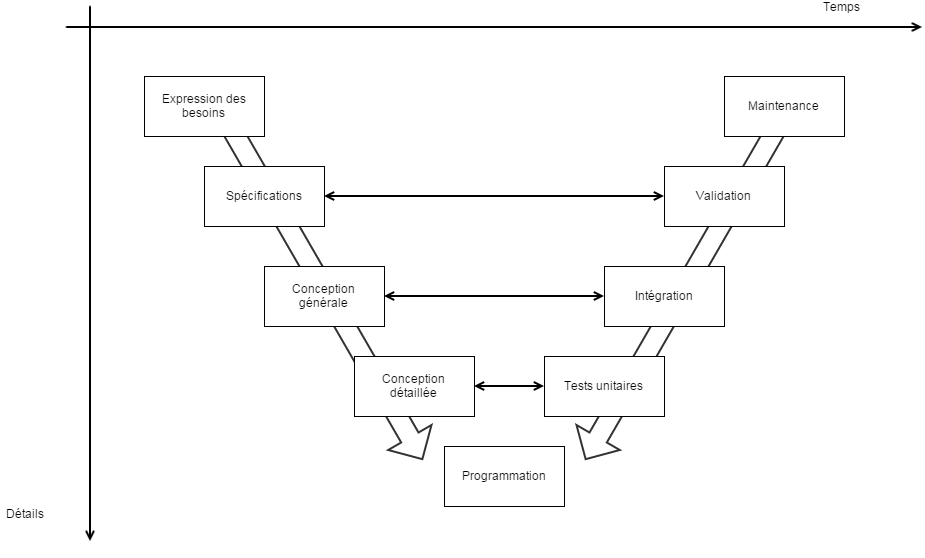
\includegraphics[keepaspectratio=true,scale=0.8]{images/cycle_en_v.png}}
\captionof{figure}{Cycle de développement en V}\label{visina8}%      only if needed
\end{minipage}

\section{Plannification}
Voici le planning qui représente la répartition des tâches durant mon stage :\\\\
\noindent%
\begin{minipage}{\linewidth}% to keep image and caption on one page
\makebox[\linewidth]{%        to center the image
  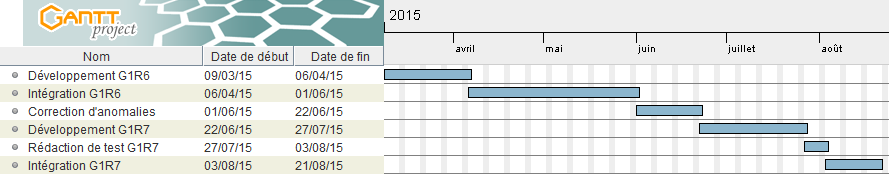
\includegraphics[keepaspectratio=true,scale=0.8]{images/gant.png}}
\captionof{figure}{Planning des tâches réalisées}\label{visina8}%      only if needed
\end{minipage}
\chapter{Travail réalisé}
Je suis arrivé sur le projet lorsque la version G1R6 étais à la fin de la phase de programmation. J'ai participé un peu à la programmation, à la phase d'intégration et de maintenance.
\\J'ai pu commencer la version G1R7 de la rédaction des spécifications jusqu'à l'intégration.
\section{Développement}
\subsection{Version G1R6}
On m'a rapidement permis de développer sur le projet. La première tâche consisté à externaliser des paramètres de configuration concernant le zoom, la projection et la minicarte qui se trouve "en dur" dans l'application.
\\Cette première tâche de développement m'a permis de mieux comprendre le fonctionnement du projet car j'ai du modifier les trois parties de l'application :\\
\begin{itemize}
\item La base de données (gfi-bdd). En insérant de nouvelles données dans la table de configuration
\item Le backoffice (gfi-back). En faisant le Mapping\footnote{Association des données en base à des objets en programmation} des données.
\item Le frontoffice (gfi-front). En supprimant les données de configuration "en dur" dans le programme et en envoyant les bonnes commandes au serveur pour récupérer les paramètres de configurations présents en base de données.\\
\end{itemize}
J'ai posé beaucoup de questions à l'équipe de développement pour valider mon travail.
\\ Ensuite j'ai eu en charge de vérifier si le paramètre de projection était bien transmis aux  \textit{Toolboxs\footnote{Les Toolboxs sont des servlets Java, ce sont des extensions des fonctions du serveur de base.}} (gfi-back) et si elles étaient bien aiguillés en fonction de ce paramètre de projection.
Pour cela j'ai du vérifier les requêtes envoyées par le client lors de l'appel de la Toolbox et vérifier dans le backoffice si le paramète était bien transmis et vers la bonne servlet en analysant ce qui était retourné.

\subsection{Version G1R7}
Lors de la phase de développement de la version G1R7 j'avais beaucoup plus d'expérience sur le projet et je n'ai pas eu de  gros problèmes à développer ce qui été demander et j'avais déjà les idées sur l'implémentation de ce que je devais faire.
\\En effet je me suis occupé du widget \textit{Publication de Schéma Directeur} (gfi-front, gfi-back, gfi-data) où j'ai ajouté le champs opérateur au niveau de la base de données et de l'IHM. Puis j'ai modifier les commandes de selections, d'extraction et d'impression pour qu'elles se réalise avec un filtrage sur le champ opérateur.
\\\\
\noindent%
\begin{minipage}{\linewidth}% to keep image and caption on one page
\makebox[\linewidth]{%        to center the image
  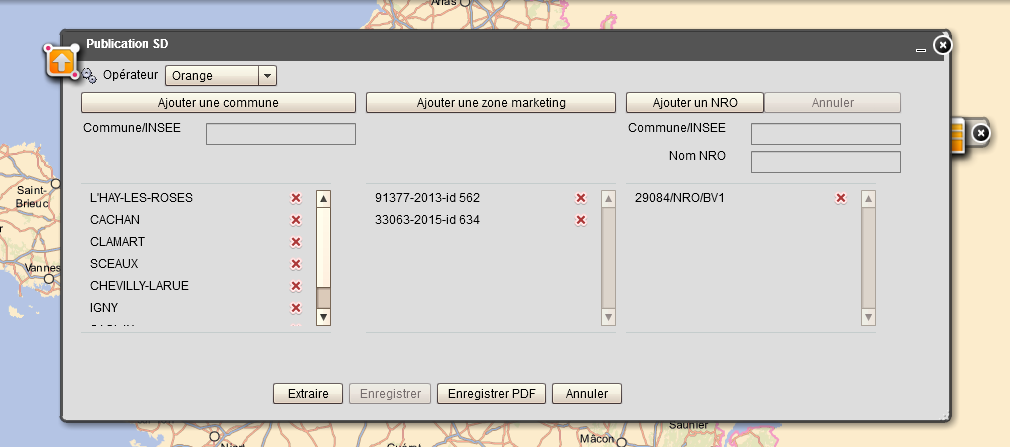
\includegraphics[keepaspectratio=true,scale=0.5]{images/publicationSD.png}}
\captionof{figure}{Widget publication SD}\label{visina8}%      only if needed
\end{minipage}\\

Je me suis ensuite occupé du \textit{programme de copie de données} (gfi-expl), qui permet de copier des données FTTH d'une commune à une autre.
\\J'ai ajouté une contrainte lié à la configuration des RIP : si la commune d'export n'a pas de configuration RIP alors elle prend pour valeur la configuration RIP de la table source.

\section{Intégration}
Je parlerais des tests d'integration, leurs niveau d'importance, le système de vagues, et un exemple de passage
\section{Corrections d'anomalies}
Je parlerais de comment on corrige une anomalie et un exemple.
